% Options for packages loaded elsewhere
\PassOptionsToPackage{unicode}{hyperref}
\PassOptionsToPackage{hyphens}{url}
\documentclass[
]{article}
\usepackage{xcolor}
\usepackage[margin=1in]{geometry}
\usepackage{amsmath,amssymb}
\setcounter{secnumdepth}{5}
\usepackage{iftex}
\ifPDFTeX
  \usepackage[T1]{fontenc}
  \usepackage[utf8]{inputenc}
  \usepackage{textcomp} % provide euro and other symbols
\else % if luatex or xetex
  \usepackage{unicode-math} % this also loads fontspec
  \defaultfontfeatures{Scale=MatchLowercase}
  \defaultfontfeatures[\rmfamily]{Ligatures=TeX,Scale=1}
\fi
\usepackage{lmodern}
\ifPDFTeX\else
  % xetex/luatex font selection
\fi
% Use upquote if available, for straight quotes in verbatim environments
\IfFileExists{upquote.sty}{\usepackage{upquote}}{}
\IfFileExists{microtype.sty}{% use microtype if available
  \usepackage[]{microtype}
  \UseMicrotypeSet[protrusion]{basicmath} % disable protrusion for tt fonts
}{}
\makeatletter
\@ifundefined{KOMAClassName}{% if non-KOMA class
  \IfFileExists{parskip.sty}{%
    \usepackage{parskip}
  }{% else
    \setlength{\parindent}{0pt}
    \setlength{\parskip}{6pt plus 2pt minus 1pt}}
}{% if KOMA class
  \KOMAoptions{parskip=half}}
\makeatother
\usepackage{longtable,booktabs,array}
\usepackage{calc} % for calculating minipage widths
% Correct order of tables after \paragraph or \subparagraph
\usepackage{etoolbox}
\makeatletter
\patchcmd\longtable{\par}{\if@noskipsec\mbox{}\fi\par}{}{}
\makeatother
% Allow footnotes in longtable head/foot
\IfFileExists{footnotehyper.sty}{\usepackage{footnotehyper}}{\usepackage{footnote}}
\makesavenoteenv{longtable}
\usepackage{graphicx}
\makeatletter
\newsavebox\pandoc@box
\newcommand*\pandocbounded[1]{% scales image to fit in text height/width
  \sbox\pandoc@box{#1}%
  \Gscale@div\@tempa{\textheight}{\dimexpr\ht\pandoc@box+\dp\pandoc@box\relax}%
  \Gscale@div\@tempb{\linewidth}{\wd\pandoc@box}%
  \ifdim\@tempb\p@<\@tempa\p@\let\@tempa\@tempb\fi% select the smaller of both
  \ifdim\@tempa\p@<\p@\scalebox{\@tempa}{\usebox\pandoc@box}%
  \else\usebox{\pandoc@box}%
  \fi%
}
% Set default figure placement to htbp
\def\fps@figure{htbp}
\makeatother
\setlength{\emergencystretch}{3em} % prevent overfull lines
\providecommand{\tightlist}{%
  \setlength{\itemsep}{0pt}\setlength{\parskip}{0pt}}
\usepackage{bookmark}
\IfFileExists{xurl.sty}{\usepackage{xurl}}{} % add URL line breaks if available
\urlstyle{same}
\hypersetup{
  pdftitle={Tau Expression in Response to ProNGF Treatment in BFCNs},
  hidelinks,
  pdfcreator={LaTeX via pandoc}}

\title{Tau Expression in Response to ProNGF Treatment in BFCNs}
\author{}
\date{\vspace{-2.5em}March 04, 2026}

\begin{document}
\maketitle

{
\setcounter{tocdepth}{2}
\tableofcontents
}
\section{Background}\label{background}

\subsection{Published Context}\label{published-context}

ProNGF --- the precursor form of Nerve Growth Factor --- was recently shown to drive
\textbf{retrograde axonal degeneration} of basal forebrain cholinergic neurons (BFCNs)
through the p75\textsuperscript{NTR} receptor and induction of amyloid precursor protein (APP).

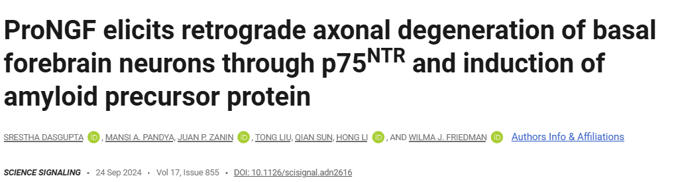
\includegraphics[width=1\linewidth]{figs/SciSignaling_header}

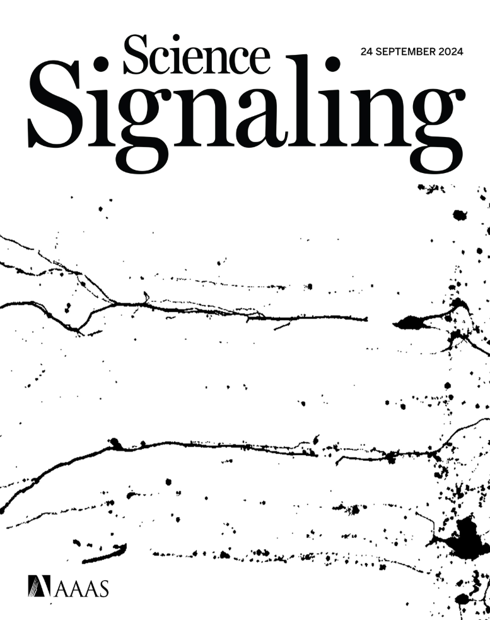
\includegraphics[width=1\linewidth]{figs/SciSignaling_cover}

\begin{center}\rule{0.5\linewidth}{0.5pt}\end{center}

\subsection{The Mechanism}\label{the-mechanism}

ProNGF acts selectively on axons, triggering a cascade that leads to both
\textbf{axon degeneration} and \textbf{cell death}:

\begin{itemize}
\tightlist
\item
  Axon-specific proNGF → p75\textsuperscript{NTR} activation
\item
  ↑ Nascent protein synthesis in axons, including \textbf{APP}
\item
  APP↑ → Ca²⁺ increase → Calpain activation
\item
  Concurrent retrograde p-JNK/JNK signalling → cell death
\end{itemize}

\begin{center}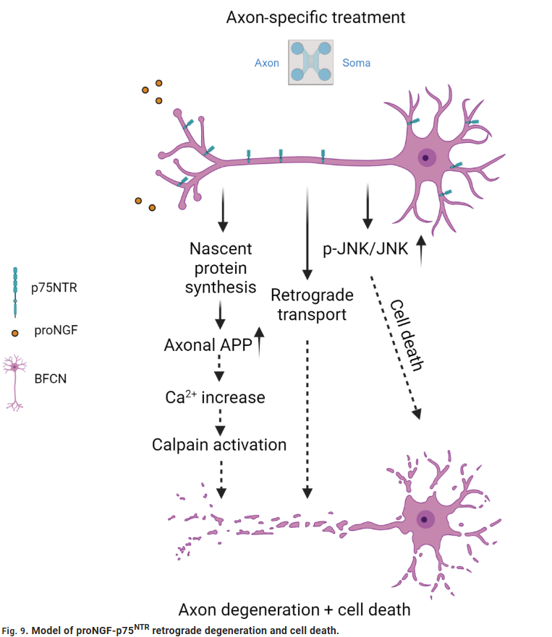
\includegraphics[width=0.55\linewidth]{figs/SciSignaling_mechanism} \end{center}

\begin{center}\rule{0.5\linewidth}{0.5pt}\end{center}

\subsection{Prior Lab Data --- Ingenuity Pathway Analysis (IPA)}\label{prior-lab-data-ingenuity-pathway-analysis-ipa}

To identify which upstream regulators are activated by axonal proNGF treatment,
BFCNs were cultured in \textbf{filter chambers} that physically separate axons from
cell bodies.

\begin{itemize}
\tightlist
\item
  Axons were treated with proNGF for \textbf{30 minutes}
\item
  Newly synthesised proteins were labelled with \textbf{O-propargyl-puromycin (OPP)}
\item
  After a \textbf{2-hour labelling window}, axonal lysates were collected and analysed
\end{itemize}

IPA of the axonal proteome revealed \textbf{MAPT (tau)} and \textbf{APP} as the top
upstream regulators (\emph{p} = 4.35×10⁻⁷⁰ and 4.83×10⁻³⁶, respectively),
with predicted downstream effects on cell death and necrosis.

\begin{center}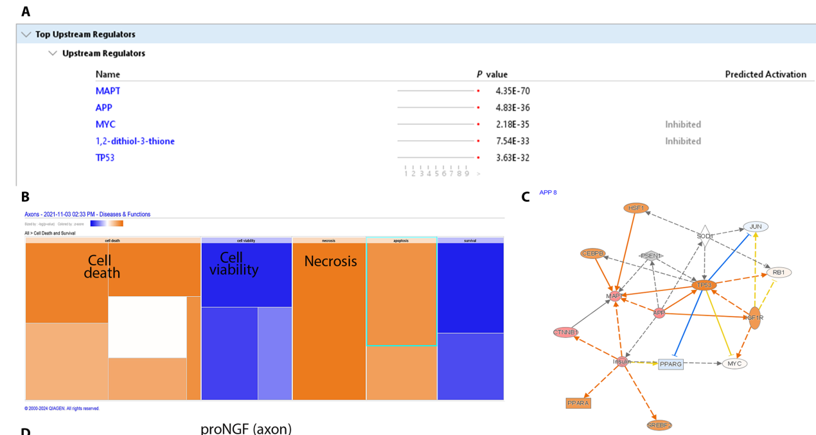
\includegraphics[width=0.75\linewidth]{figs/SciSignaling_IPA} \end{center}

\begin{center}\rule{0.5\linewidth}{0.5pt}\end{center}

\subsection{Rationale for This Study}\label{rationale-for-this-study}

The IPA data pointed to \textbf{tau (MAPT)} as a central upstream regulator of the
axonal response to proNGF --- yet the specific changes in tau protein expression
and phosphorylation state had not been characterised.

\textbf{This study asks:}

\begin{quote}
Does proNGF treatment alter \textbf{total tau} and \textbf{phospho-tau} levels
in the axon and soma compartments of BFCNs?
\end{quote}

We used Western blotting with antibodies targeting three phosphorylation sites ---
\textbf{pThr181}, \textbf{pSer202/pThr205 (AT8)}, and \textbf{pSer622} --- alongside pan-tau,
to capture both the abundance and phosphorylation state of tau across
compartments.

\section{Total Tau Increase in Response to ProNGF Treatment}\label{total-tau-increase-in-response-to-prongf-treatment}

\subsection{Overview}\label{overview}

ProNGF treatment was applied to compartmentalized basal forebrain cholinergic neuron cultures.

Western blotting was used to assess changes in \textbf{total Tau} and \textbf{phospho-Tau} protein levels across soma and axon compartments.

\begin{center}\rule{0.5\linewidth}{0.5pt}\end{center}

\subsection{Tau Phosphorylation Sites for Antibodies used}\label{tau-phosphorylation-sites-for-antibodies-used}

In this research, I quantified tau phosphorylation using three antibodies that report distinct tau states:

\begin{itemize}
\item
  \textbf{pThr181 (p-tau181)}: commonly used biomarker-associated phosphorylation site that tracks Alzheimer's disease-related tau pathology in CSF and plasma and is widely used for staging/stratification.\\
  (Context review: \url{https://pmc.ncbi.nlm.nih.gov/articles/PMC10839341/})
  Key kinases: GSK-3β, CDK5.
\item
  \textbf{AT8 (pSer202/pThr205)}: canonical neuropathology epitope used to detect early and established pathological tau (pre-tangles/tangles) in tissue; often treated as a marker of disease-associated tau phosphorylation.\\
  (Epitope/usage context: \url{https://www.alzforum.org/alzantibodies/tau-at8-phospho-tau-ser-202-thr-205})
  Key kinases: GSK-3β, MAPK, CDK5.
\item
  \textbf{pSer622}: a C-terminal tau site sometimes assessed in biochemical studies; interpretation can depend on antibody specificity and isoform context, and is typically considered alongside broader phosphorylation patterns rather than as a standalone ``core biomarker'' site.\\
  (Phosphorylation landscape context: \url{https://pmc.ncbi.nlm.nih.gov/articles/PMC10839341/})
  Key kinases: Casein kinase 1 and 2, GSK-3β.
\end{itemize}

\begin{center}\rule{0.5\linewidth}{0.5pt}\end{center}

\subsection{Phosphorylation Patterns of Tau}\label{phosphorylation-patterns-of-tau}

\begin{figure}
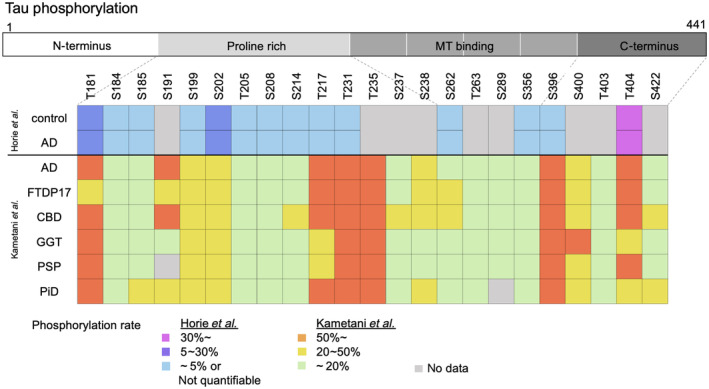
\includegraphics[width=0.8\linewidth]{figs/external_pTau_FEB4-14-181-g005} \caption{The figure shows the phosphorylation sites of tau identified in each disease and the frequency (Horie et al. and Kametani et al.)}\label{fig:fig-phospho-patterns}
\end{figure}

\begin{center}\rule{0.5\linewidth}{0.5pt}\end{center}

\subsection{Composite Western Blot --- All Compartments}\label{composite-western-blot-all-compartments}

\begin{figure}
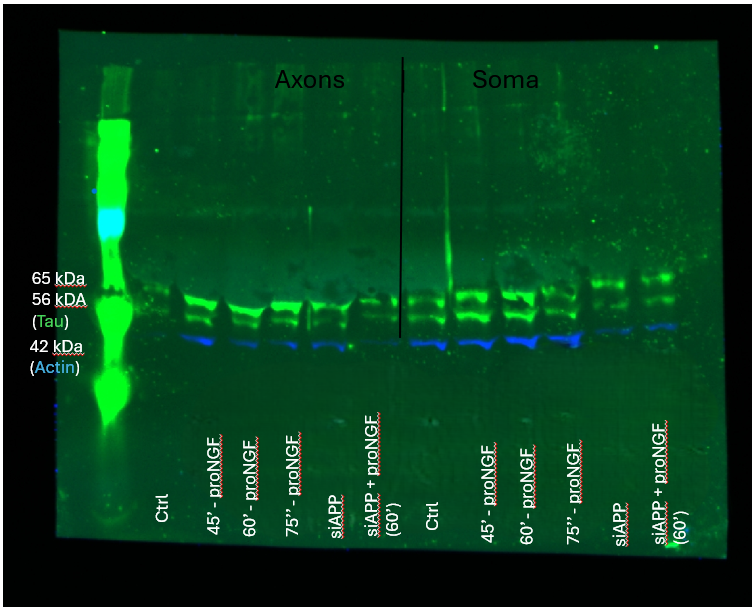
\includegraphics[width=0.8\linewidth]{figs/ColoredLabeledWB_Feb12} \caption{Western blot analysis of Tau and actin expression. Composite image.}\label{fig:fig-composite-wb}
\end{figure}

\begin{center}\rule{0.5\linewidth}{0.5pt}\end{center}

\subsection{Representative Composite Image}\label{representative-composite-image}

\begin{figure}
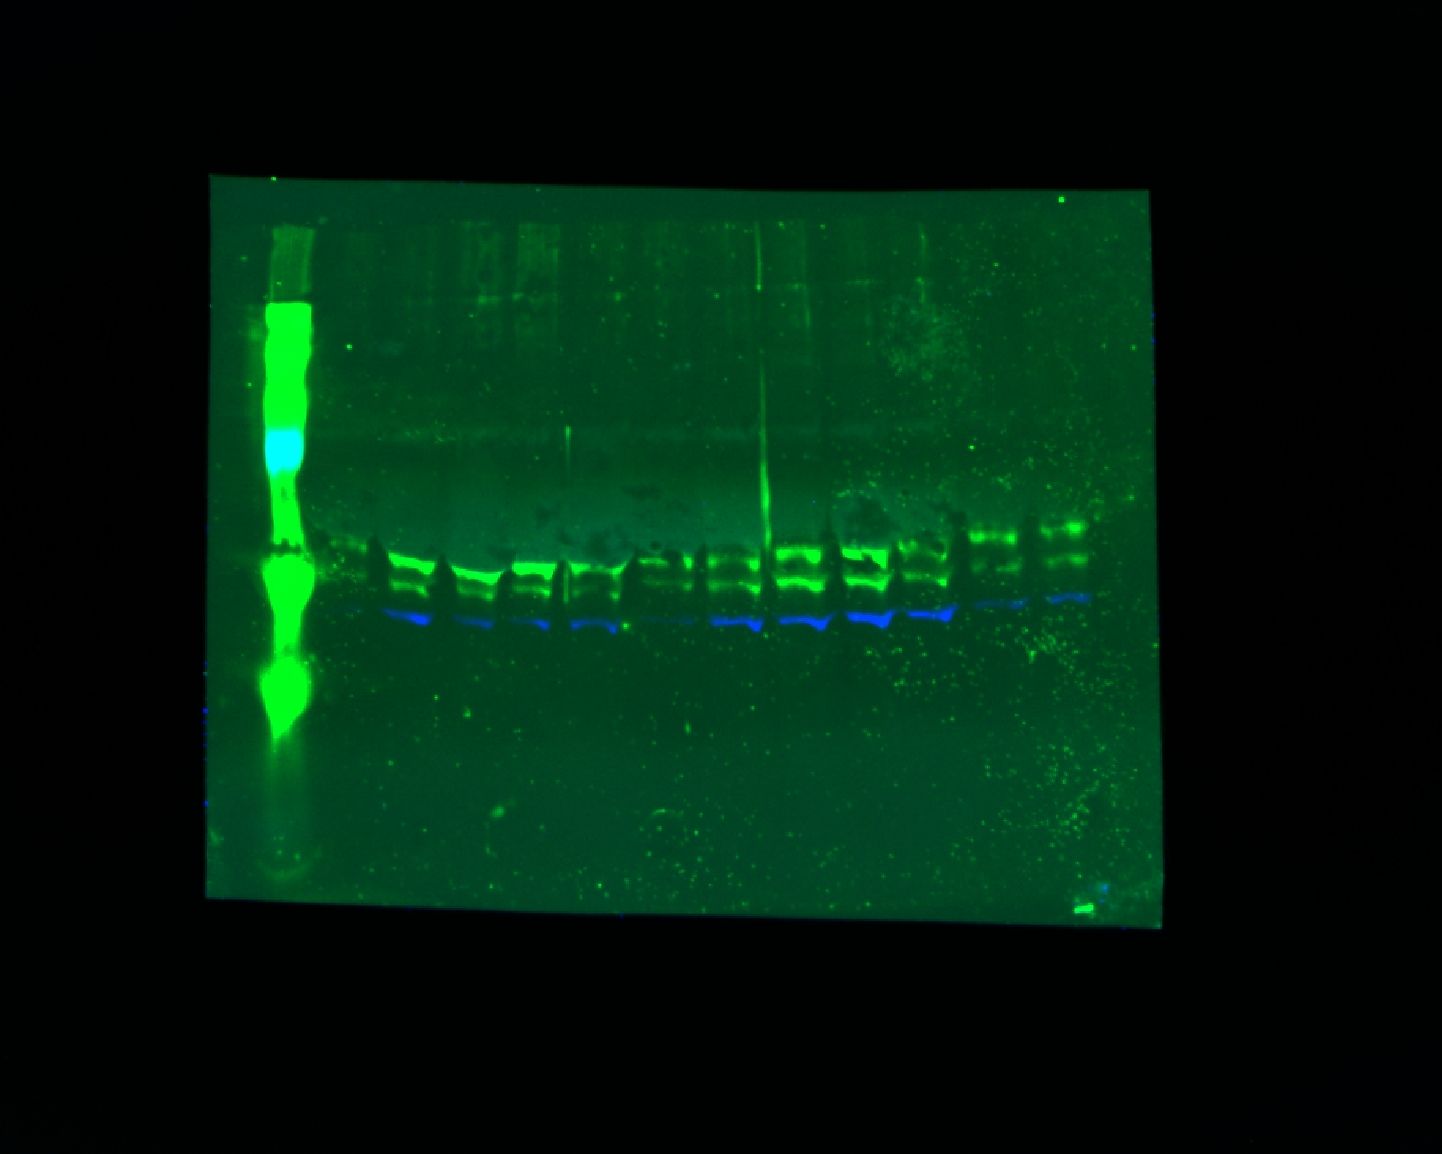
\includegraphics[width=0.8\linewidth]{figs/ELINA_2026-02-12_12h52m48s_Composite_} \caption{Representative composite image showing actin (blue) and Tau (green).}\label{fig:fig-actin-tau}
\end{figure}

\begin{center}\rule{0.5\linewidth}{0.5pt}\end{center}

\subsection{Green Channel --- Actin \& Phospho-Tau (800CW)}\label{green-channel-actin-phospho-tau-800cw}

\begin{figure}
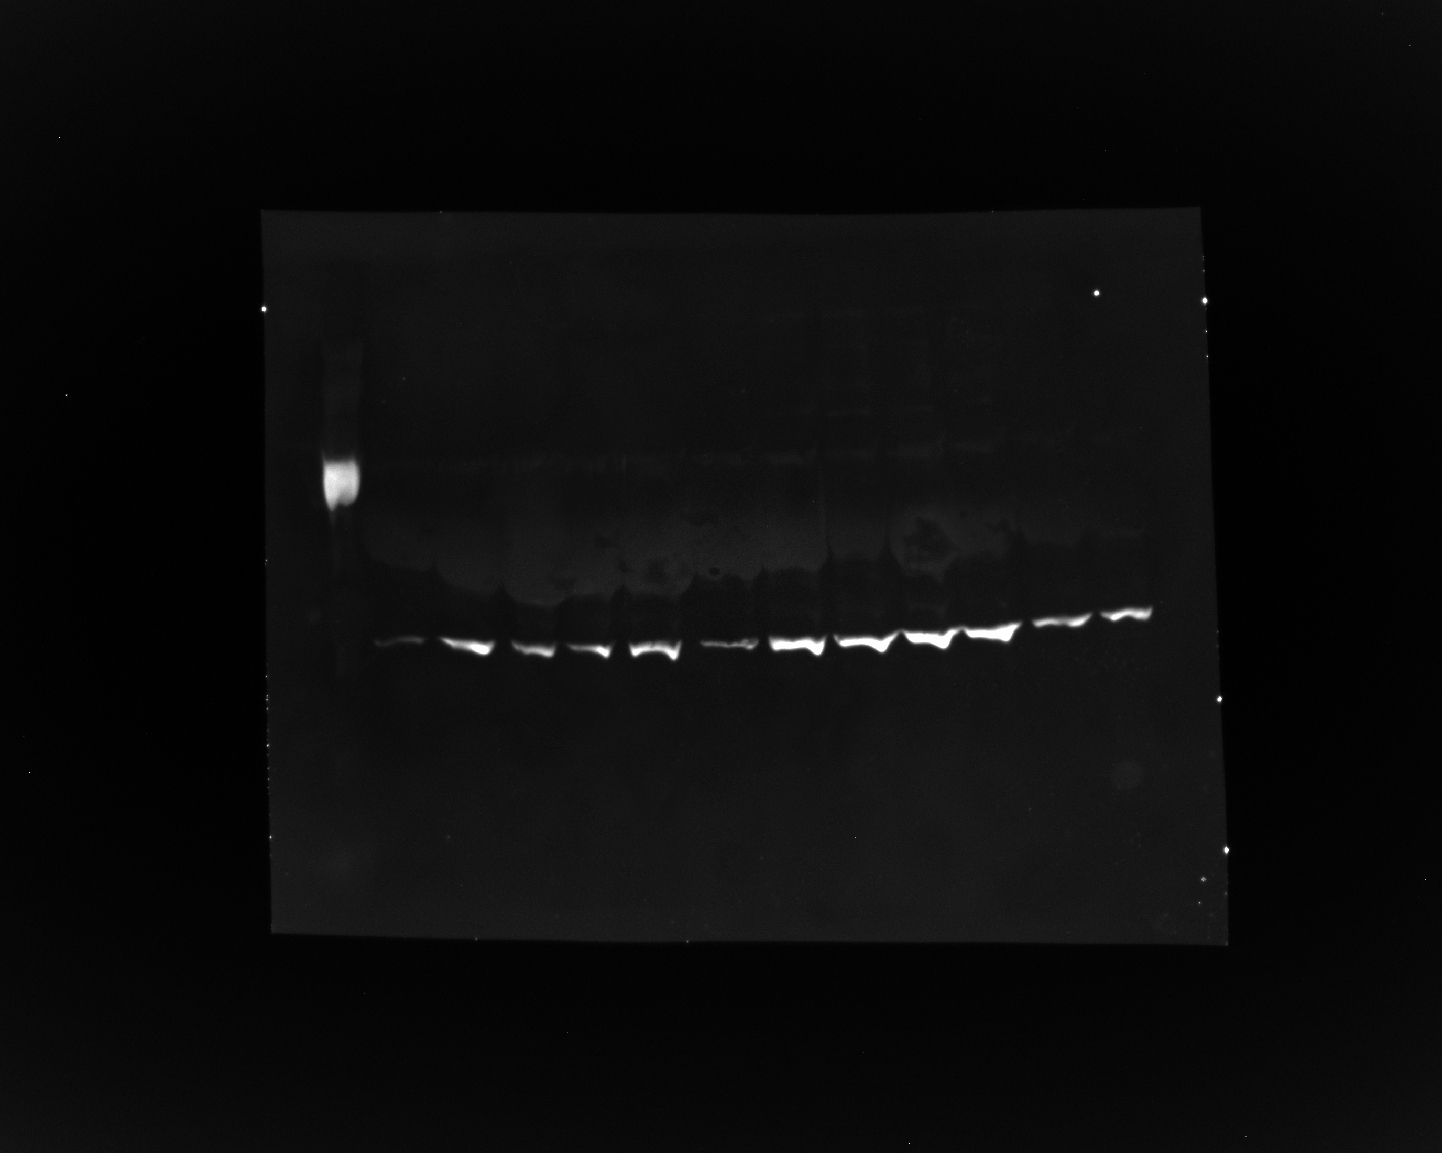
\includegraphics[width=0.8\linewidth]{figs/ELINA_2026-02-05_12h18m48s_IRDye_800CW_} \caption{Green channel image showing actin (mouse) and phospho-Tau (rabbit; pSer202/pThr205).}\label{fig:fig-actin-ptau-800}
\end{figure}

\begin{center}\rule{0.5\linewidth}{0.5pt}\end{center}

\subsection{Red Channel --- Total Tau (pan-Tau; Rb-237)}\label{red-channel-total-tau-pan-tau-rb-237}

\begin{figure}
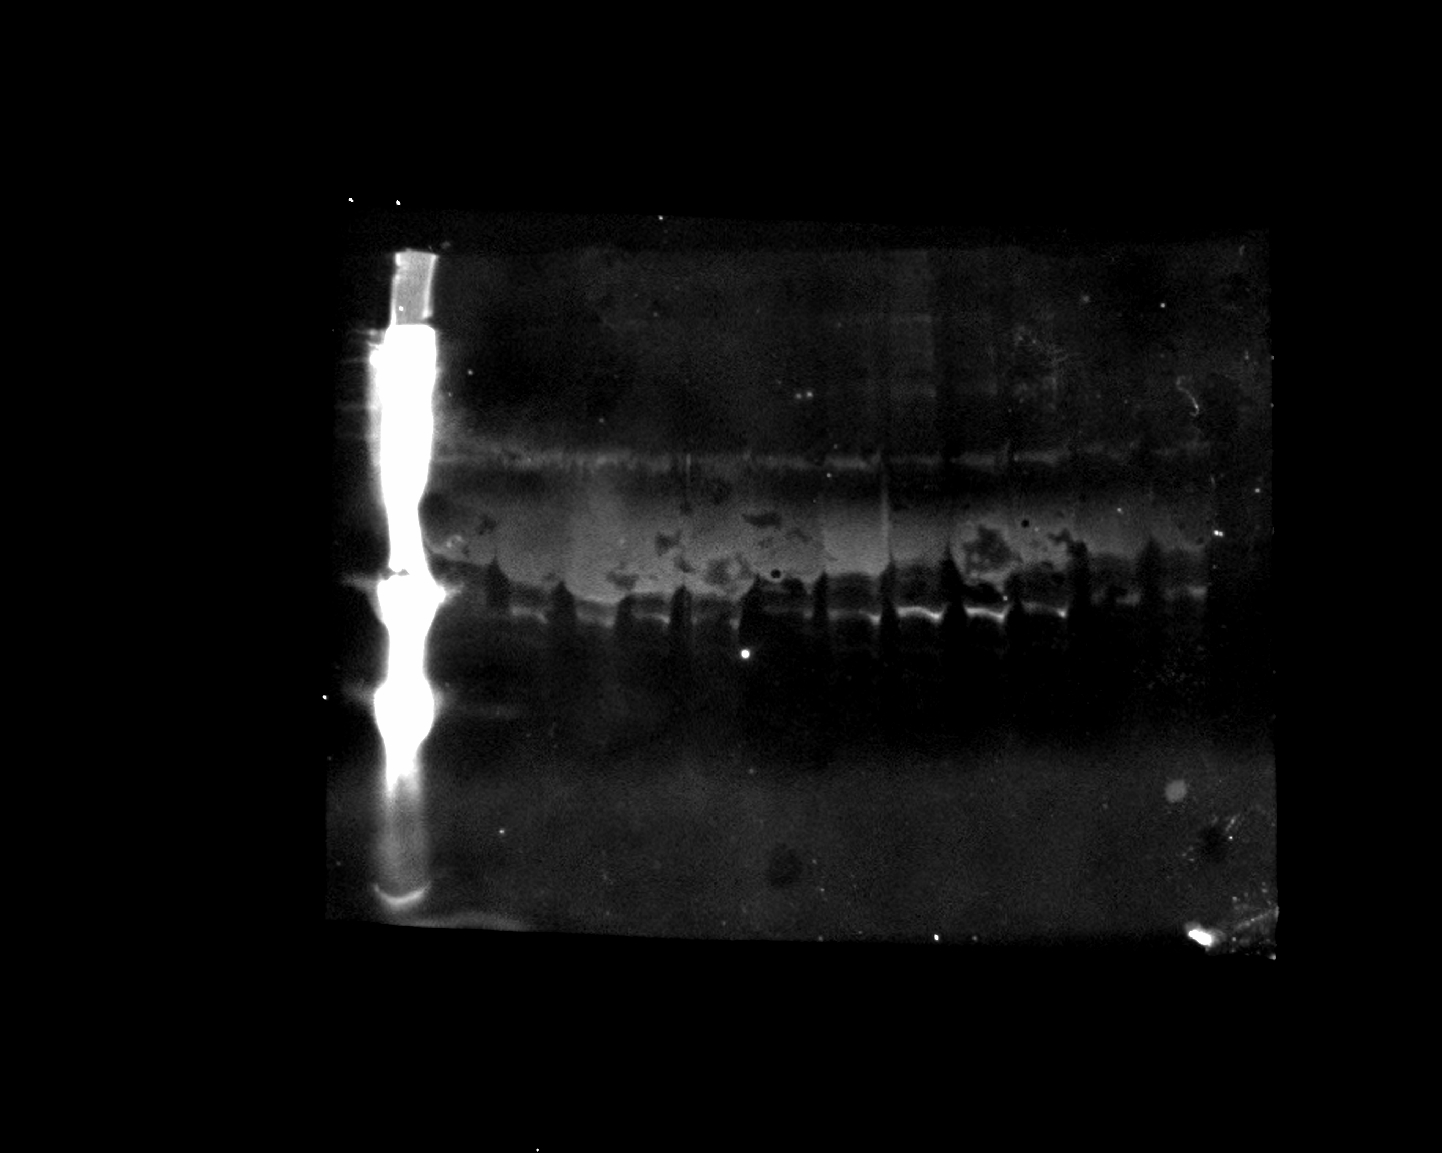
\includegraphics[width=0.8\linewidth]{figs/ELINA_2026-02-06_13h04m41s_IRDye_680RD_} \caption{Red channel image showing total Tau (pan-Tau; Rb-237).}\label{fig:fig-tau-680}
\end{figure}

\section{Soma-Only Repeat Western Blot}\label{soma-only-repeat-western-blot}

\subsection{Overview}\label{overview-1}

A repeat Western blot was performed on \textbf{soma-only} fractions from the same samples as above.

Targets: \textbf{phospho-Tau (pSer622)}, \textbf{pan-Tau}, and \textbf{actin}.

\begin{center}\rule{0.5\linewidth}{0.5pt}\end{center}

\subsection{Soma-Only Composite Western Blot}\label{soma-only-composite-western-blot}

\begin{figure}
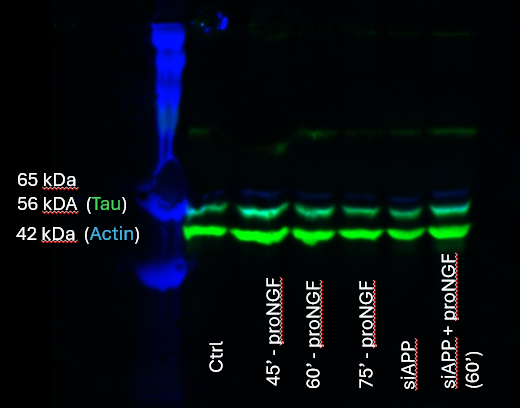
\includegraphics[width=0.8\linewidth]{figs/ColoredLabeledWB_onlySoma} \caption{Western blot analysis of phosphoTau, panTau and actin expression. Composite image.}\label{fig:fig-soma-wb}
\end{figure}

\begin{center}\rule{0.5\linewidth}{0.5pt}\end{center}

\subsection{Red Channel --- Phospho-Tau at Ser622 (680RD)}\label{red-channel-phospho-tau-at-ser622-680rd}

\begin{figure}
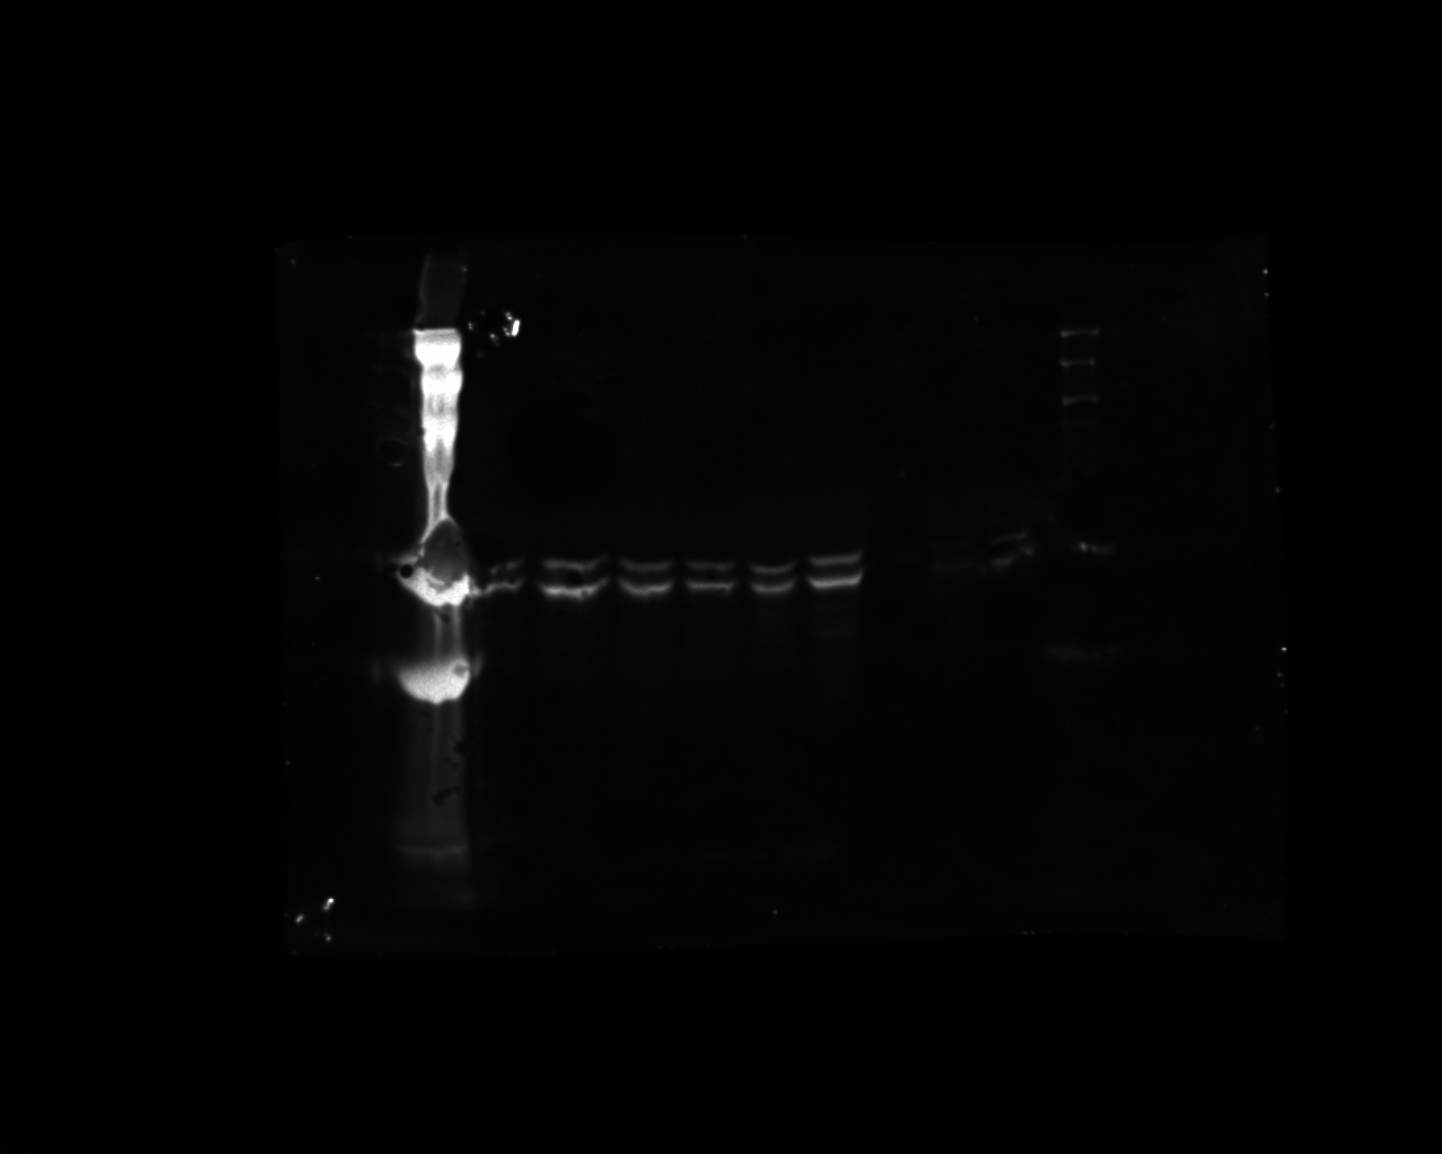
\includegraphics[width=0.8\linewidth]{figs/ELINA_2026-02-11_13h52m00s_IRDye_680RD_} \caption{Red channel image showing phospho-Tau at Ser622 (pSer622).}\label{fig:fig-ptau-ser622}
\end{figure}

\begin{center}\rule{0.5\linewidth}{0.5pt}\end{center}

\subsection{Composite --- pSer622 \& Pan-Tau}\label{composite-pser622-pan-tau}

\begin{figure}
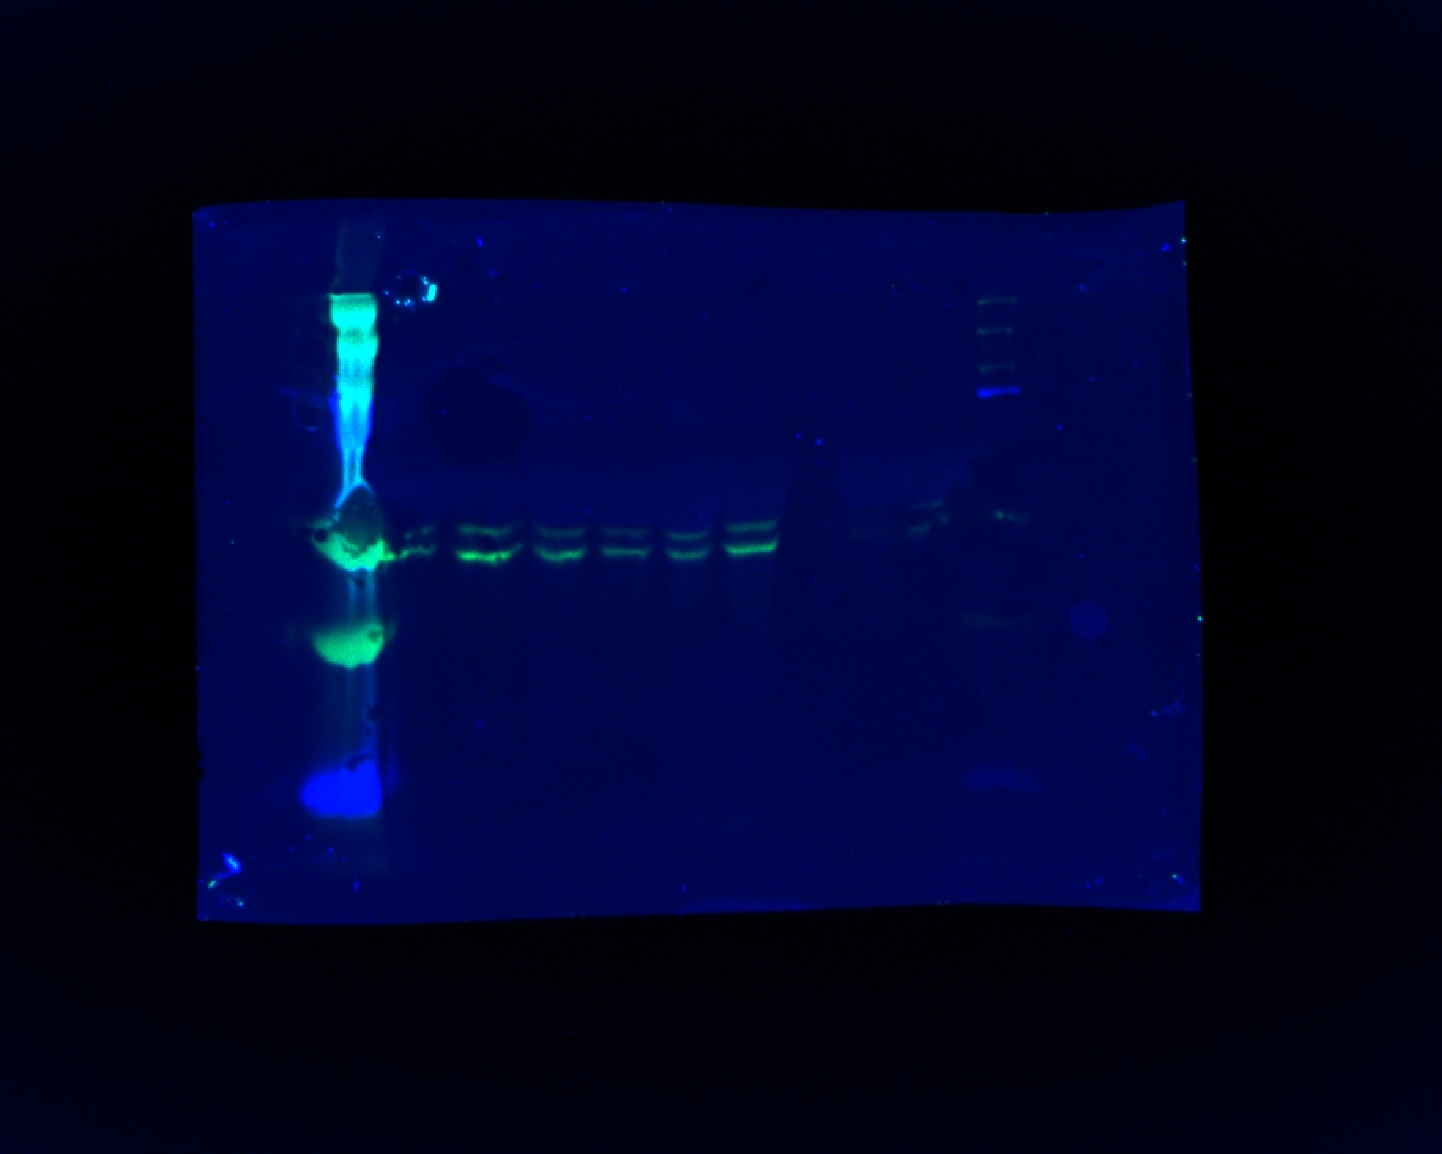
\includegraphics[width=0.8\linewidth]{figs/ELINA_2026-02-13_10h47m12s_Composite_} \caption{Composite image: phospho-Tau at Ser622 (red channel) and pan-Tau (green channel; Red antibody = Rabbit, Green antibody = Mouse).}\label{fig:fig-ptau-composite}
\end{figure}

\section{Summary}\label{summary}

\subsection{Key Findings}\label{key-findings}

\begin{itemize}
\tightlist
\item
  IPA of axonal lysates after proNGF treatment identified \textbf{MAPT (tau)} and \textbf{APP}
  as the top upstream regulators, motivating a direct biochemical assessment of tau
\item
  ProNGF treatment induces changes in \textbf{total Tau} levels detectable by Western blot
\item
  Phosphorylation at \textbf{pSer202/pThr205} and \textbf{pSer622} sites assessed across compartments
\item
  Soma-only repeat blots confirm signal specificity in the \textbf{cell body fraction}
\end{itemize}

\textbf{Next steps:} Quantification of band intensities and normalization to actin loading control

\end{document}
